\subsection{Reserved results and exact checks}

\label{sec:acceleration-results}

The frozen comparison contains 720 planned records across twelve family instances, two target-batch sizes, six methods and five repetitions. We executed 616 trials and obtained 590 exact completions; the remaining 26 executed trials exceeded a resource limit or failed to complete. The early-stop rule left 104 repetitions unexecuted. These skipped records contain no timing measurement. The retained inputs, policy choices, successful reductions and failure records accompany the data release~\cite{KiraNativeAccelerationData}.

Validation selected the complete target expression with threshold $\tau=0.01$. This configuration and both trained checkpoints remained fixed during the reserved tests. Each method used the same master basis and targets in a batch.

For the three controls, restricted native Kira produced 105 exact completions, 3 failed trials and 12 skipped repetitions, the target-bound control produced 100 exact completions, 4 failed trials and 16 skipped repetitions, and the full candidate-pool control produced 105 exact completions, 3 failed trials and 12 skipped repetitions. These counts describe the bounded experiment and do not measure whether an unlimited calculation would complete.

Successful restricted-native trials took 10.54--112.46 seconds for the complete checked calculation. This range includes different family instances, target-batch sizes and CPU models. The paired ratios compare methods on the same node within each batch.

For the learned methods, the learned seed filter produced 100 exact completions, 4 failed trials and 16 skipped repetitions, the compiled row policy produced 105 exact completions, 3 failed trials and 12 skipped repetitions, and the combined method produced 75 exact completions, 9 failed trials and 36 skipped repetitions. Completed seed and combined trials used the standard fallback 30 and 50 times, respectively.

Every completed final expression matched its recorded rational master coefficients. The independent audit performed 67,920 additional master-coefficient sample checks and 65,355 exact-row sample checks. It checked 11,405 compiled model choices and 10,380 forced source actions. Trace checks cover completed native attempts; 55 failed attempts had incomplete traces. The final coefficient checks still apply to any successful fallback. Input and checkpoint hashes agree with the values frozen before testing.

\subsection{Complete reduction time and algebraic work}

For each family and batch size, we take the median of five successful repetitions. We then form the ratio of learned time to control time and report the geometric mean across complete paired batches. A ratio below one means a lower measured time. We resample complete kinematic groups 10,000 times to obtain descriptive 95\% intervals, keeping related profiles and batch sizes together. These intervals describe the completed subset of this small collection; failed and skipped trials remain in the completion counts above.

Restricted native Kira completed all five repetitions in 1 batches where the learned seed filter did not, while the learned seed filter completed all five repetitions in 0 batches where that control did not.

The learned seed filter has a complete-time ratio of 1.295 (descriptive 95\% interval 1.156--1.542; 20 batches) against restricted native Kira. Its native-calculation subtotal, including seed prediction when used, has ratio 1.400 (descriptive 95\% interval 1.201--1.816; 20 batches). The subtotal excludes input preparation, final target combination and verification, which remain included in the complete time.

Restricted native Kira completed all five repetitions in 0 batches where the compiled row policy did not, while the compiled row policy completed all five repetitions in 0 batches where that control did not.

The compiled row policy has a complete-time ratio of 1.024 (descriptive 95\% interval 0.998--1.053; 21 batches) against restricted native Kira. Its native-calculation subtotal, including seed prediction when used, has ratio 1.025 (descriptive 95\% interval 1.001--1.078; 17 batches). The subtotal excludes input preparation, final target combination and verification, which remain included in the complete time.

Restricted native Kira completed all five repetitions in 6 batches where the combined method did not, while the combined method completed all five repetitions in 0 batches where that control did not.

The combined method has a complete-time ratio of 1.983 (descriptive 95\% interval 1.575--2.476; 15 batches) against restricted native Kira. Its native-calculation subtotal, including seed prediction when used, has ratio 2.289 (descriptive 95\% interval 1.247--3.673; 8 batches). The subtotal excludes input preparation, final target combination and verification, which remain included in the complete time.

Against the target-bound control, complete-time ratios are 0.902 (descriptive 95\% interval 0.711--1.163; 20 batches), 0.712 (descriptive 95\% interval 0.597--0.864; 20 batches), 1.415 (descriptive 95\% interval 0.902--2.160; 14 batches), in seed, row and combined order. Against the full candidate-pool control, the corresponding ratios are 1.317 (descriptive 95\% interval 1.167--1.569; 20 batches), 1.040 (descriptive 95\% interval 1.016--1.061; 21 batches), 2.028 (descriptive 95\% interval 1.565--2.616; 15 batches). Each ratio uses its own complete paired cohort, so comparisons with different failure patterns can contain different batches.

\begin{figure}[htbp]
\centering
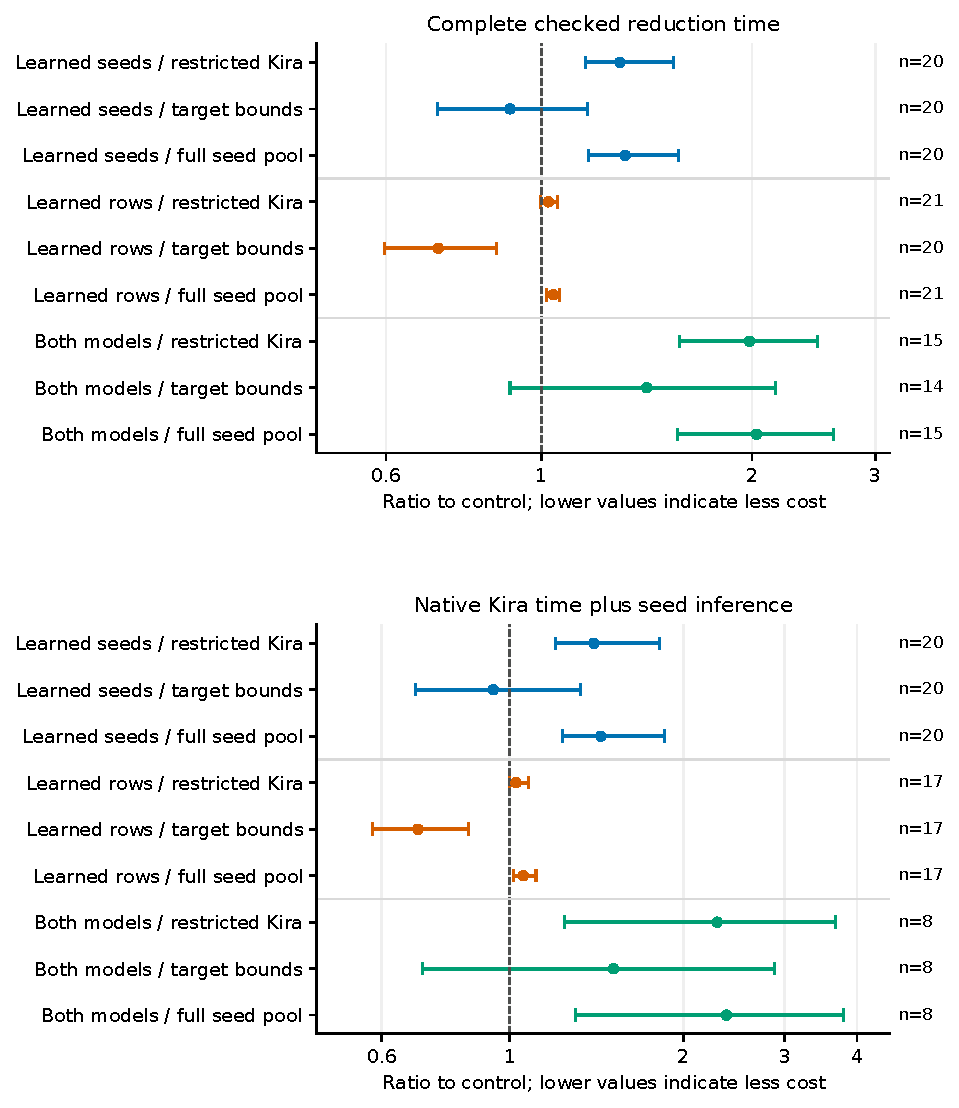
\includegraphics[width=\linewidth]{figures/native_acceleration_times.pdf}
\caption{Learned-to-control time ratios in the reserved native comparison.
The upper panel includes the complete checked reduction, and the lower panel
shows the native subprocess subtotal plus seed prediction. Points show
geometric mean ratios and lines show descriptive intervals obtained by
resampling kinematic groups. The label $n$ gives the number of paired
batches with five successful repeats for both methods.}
\label{fig:native-acceleration-time}
\end{figure}

The learned seed filter has a generated-equation ratio of 0.168 (descriptive 95\% interval 0.097--0.294; 20 batches), a selected-equation ratio of 0.982 (descriptive 95\% interval 0.797--1.205; 20 batches) and a forward-update ratio of 3.575 (descriptive 95\% interval 2.647--5.211; 20 batches) against restricted native Kira. These are counters from the native reduction passes, including completed fallback passes.

The compiled row policy has a generated-equation ratio of 1.141 (descriptive 95\% interval 1.032--1.275; 21 batches), a selected-equation ratio of 1.141 (descriptive 95\% interval 1.032--1.275; 21 batches) and a forward-update ratio of 0.905 (descriptive 95\% interval 0.840--0.972; 17 batches) against restricted native Kira. These are counters from the native reduction passes, including completed fallback passes.

The combined method has a generated-equation ratio of 0.462 (descriptive 95\% interval 0.254--0.745; 15 batches), a selected-equation ratio of 1.341 (descriptive 95\% interval 1.080--1.582; 15 batches) and a forward-update ratio of 2.363 (descriptive 95\% interval 1.041--4.534; 8 batches) against restricted native Kira. These are counters from the native reduction passes, including completed fallback passes.

Generation counters count equations reported in successive generation passes and can include repeated equations. A forward update is one committed elimination step; this count does not measure every polynomial or rational-function operation. Failed attempts can have truncated work counters, so the complete time and completion status remain the primary measures.

\begin{figure}[htbp]
\centering
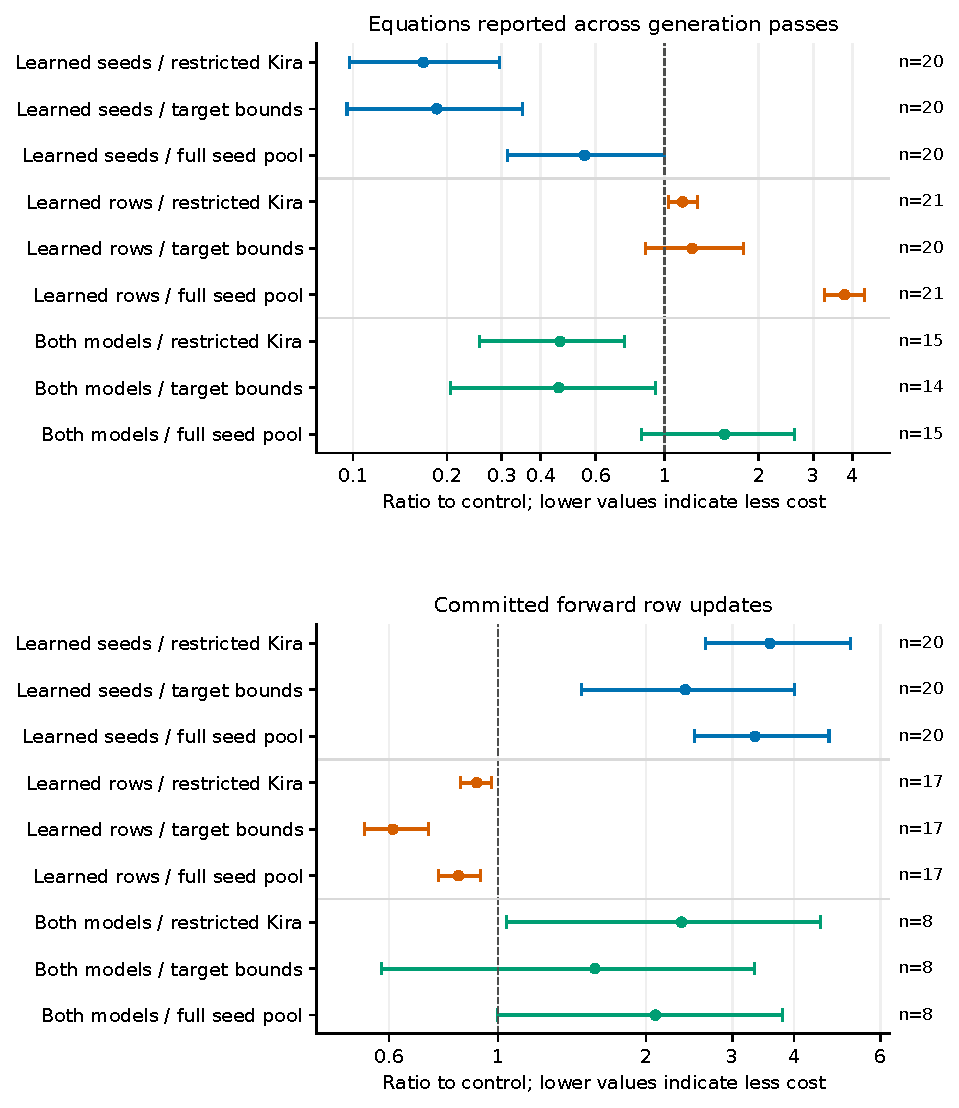
\includegraphics[width=\linewidth]{figures/native_acceleration_work.pdf}
\caption{Generated-equation and forward-update ratios on complete paired
batches. The controls and cohort labels follow
Fig.~\ref{fig:native-acceleration-time}. These counters measure reported
generation work and committed updates, while symbolic coefficient
complexity can change the cost of each update.}
\label{fig:native-acceleration-work}
\end{figure}
\FloatBarrier

\subsection{Numerical inference and scope of the result}

The compiled-model development audit checked 256 action feature vectors and 2,247 sampled coefficients. The maximum feature difference was 0, and the largest probability difference from the independent double-precision calculation was $1.41\times10^{-13}$. All selected sources agreed with the original single-precision model in these development trials. The separate maximum probability difference from that original arithmetic was $1.6\times10^{-05}$.

The largest sampled process-tree memory was 0.506 GB, and the largest trial scratch directory was 49.29 MB. The bounded runs kept their scientific records and model files on Hoffman; the report contains the derived plots and results.

The complete paired comparisons do not show a lower aggregate runtime than restricted native Kira for these learned methods. Lower inference costs alone do not ensure that the chosen seeds and rows save enough algebraic work. The new native tests cover one-loop boxes and do not establish performance on independent high-loop scattering families. The existing weights were trained to recover recorded seed sets and row choices, and Section~\ref{sec:complete-multiloop} reports a separate cost-trained policy on native Kira trajectories.
